\documentclass[border=0.8ex,svgnames,tikz]{standalone}
\usepackage{amsmath,mathtools}
\usepackage{fontspec}
\setmainfont{Source Serif 4}
\setsansfont{Source Sans 3}
\setmonofont{Source Code Pro}
\usetikzlibrary{positioning,chains}
\newcommand{\ptrcolor}{LightSlateBlue}
\newcommand{\itcolor}{IndianRed}
\begin{document}
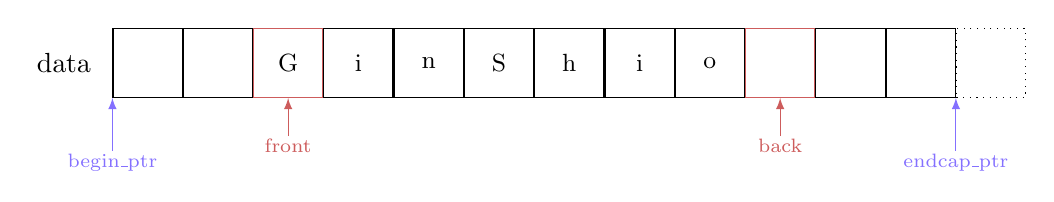
\begin{tikzpicture}
  \begin{scope}[
    node distance=0,
    every node/.style={draw,on chain,inner sep=1ex,minimum width=2.5em,minimum
      height=2.5em,font=\small},
    start chain=going right,
    ]
    % datas
    \node(begincap){};
    \node{};
    \node[draw=\itcolor](begin){G};
    \node{i};
    \node{n};
    \node{S};
    \node{h};
    \node{i};
    \node{o};
    \node[draw=\itcolor](end){};
    \node{};
    \node{};
    \node[dotted](endcap){};
  \end{scope}
  \begin{scope}[
    every path/.style={draw,>=latex},
    every node/.style={draw=none,inner sep=0.2ex,font=\scriptsize},
    ]
    \path[color=\ptrcolor,text=\ptrcolor]
    (begincap.west) ++(0,-3.6em) node{begin\_ptr} edge[->] (begincap.south west)
    (endcap.west) ++(0,-3.6em) node{endcap\_ptr} edge[->] (endcap.south west);
    \path[color=\itcolor,text=\itcolor]
    (begin) ++(0,-3em) node{front} edge[->] (begin)
    (end) ++(0,-3em) node{back} edge[->] (end);
  \end{scope}
  \node[left=1ex of begincap]{data};
\end{tikzpicture}
\end{document}
